
%(BEGIN_QUESTION)
% Copyright 2012, Tony R. Kuphaldt, released under the Creative Commons Attribution License (v 1.0)
% This means you may do almost anything with this work of mine, so long as you give me proper credit

One laborer working on the top of a building uses a manual hoist to lift 10 gallons of water 30 feet up from ground level, while a second laborer uses an electric pump to do the same:

$$\includegraphics[width=15.5cm]{i02612x01.eps}$$

First, calculate the amount of work needed to lift 10 gallons up to the same roof.  Then, calculate the time required for the pump to do this job, assuming a rating of 1.5 horsepower.

\underbar{file i02612}
%(END_QUESTION)





%(BEGIN_ANSWER)

Calculating the work in raising 10 gallons of water 30 feet up:

$$\left( 10 \hbox{ gal} \over 1 \right) \left(231 \hbox{ in}^3 \over 1 \hbox{ gal} \right) \left(1 \hbox{ ft}^3 \over 1728 \hbox{ in}^3 \right) \left(62.4 \hbox{ lb} \over \hbox{ ft}^3 \right) = 83.42 \hbox{ lb of water in 10 gallons}$$

Now, knowing both the force (83.42 lb) and the displacement (30 ft), we may calculate the work done:

$$W = F x \cos \theta$$

$$W = (83.42 \hbox{ lb})(30 \hbox{ ft})(\cos 0^o) = 2502.5 \hbox{ ft-lb of work}$$

\vskip 20pt

Now, since we know that 1 horsepower is 550 ft-lbs of work {\it per second of time}, we may take this total amount of work (2502.5 ft-lb) and divide by the pump's power in foot-pounds per second to arrive at an answer for time in seconds.  Since we know the pump's power rating is 1.5 horsepower, it means it is capable of doing 825 ft-lb of work per second:

$$t = {W \over P} = {2502.5 \hbox{ ft-lb} \over 825 \hbox{ ft-lb/s}}$$

$$t = 3.033 \hbox{ seconds}$$

%(END_ANSWER)





%(BEGIN_NOTES)


%INDEX% Physics, energy, work, power

%(END_NOTES)


